\chapter{The Container Loading Problem}
\label{sec:clp_definition}

The placement and assignment of items to larger, mostly rectangular
containers, is a well known problem in logistics and operations research, as the
potential of cost savings and efficiency gains is substantial by reducing the number
of needed containers or by fulfilling customer needs.
\gls{CLP} problems are differentiated by \citeauthor*{bortfeldt_constraints_2013} in \textit{input minimization},
where the number of needed containers is minimized, and \textit{output maximization} problems,
where the value of the associated items is maximized. The \gls{BPP} belongs to \textit{input minimization} problems
and the Knapsack Problem to \textit{output maximization}. Apart from the expected outcome of the optimization,
the characterics of the items and containers is relevant for the problem definition.Items can be either
homogenous or heterogenous sized and shaped. Further it can be differentiated between weakly and strongly
homogenous or heterogeneous, defining the degree of similarity of the items. The container is
defined as a recangular volume with a fixed size and shape, where the items have to be placed in.
Other, non rectangular, shapes are seldomly considered in the literature, as the practical relevance is
limited \footcite[cf.][pp.1--2]{bortfeldt_constraints_2013}. Multiple containers, with homogeneous
or heterogenous size, are used, whenever the volume and weight of the cargo requires it.
A possible placement of cargo into a container can be seen in Figure \ref{fig:solution-visualization}.
\begin{figure}[ht]
    \centering
    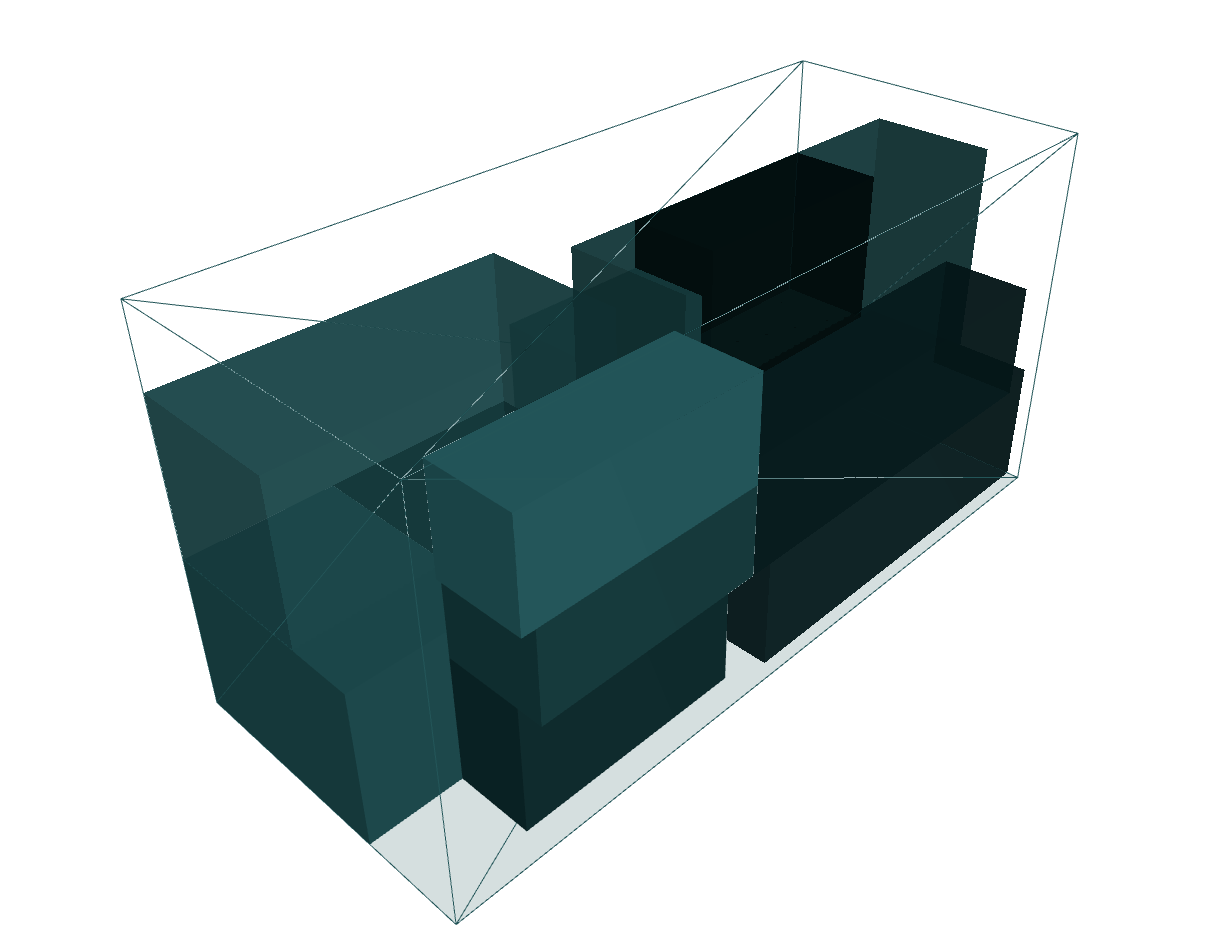
\includegraphics[width=6.3cm]{pictures/3l_cvrp_example.png}
    \caption[Visualized 3D packing with packing constraints]{Visualized 3D packing with packing constraints\footnotemark}.
    \footnotetext{CLP Visualizer from \cite{tamke_branch-and-cut_2024}}
    \label{fig:solution-visualization}
\end{figure}
\clearpage
According to \citeauthor*{bischoff_issues_1995}, the mere placement of items is insufficient
if practical requirements are not fulfilled \footcite[cf.][pp.1--2]{bischoff_issues_1995}. Building on this insight,
\citeauthor*{bortfeldt_constraints_2013} systematically categorized all constraints relevant
to the \gls{CLP} into five groups, which are presented in the following. They also distinguish between hard and soft constraints,
where hard constraints must be strictly satisfied, while soft constraints may be violated
to some extent, depending on the implementation context. \footcite[cf.][p.2]{bortfeldt_constraints_2013}.

\subsubsection{Container related constraints}
These constraints summarize all physical barriers of the container. The \textbf{load capacity} limits the aggregated
mass of all items in the container. The distribution of the weight (\textbf{load balance})
plays also an important role for safety reasons, as the cargo must not move during the transport and the container
must not tip over and is defined by the maximum weight difference between the left and right half of the container.
In the special case of trucks, uneven \textbf{axle weight} distribution can cause severe
crash consequences and need to be avoided by loading the cargo axle-friendly \footcite[cf.][pp. 849--850]{krebs_advanced_2021}.

\subsubsection{Item related constraints}
Item related constraints define the properties of the item, which are relevant
for the packing. When the container capacity is limited (\textit{output maximization}),
the \textbf{loading priority} constraint can define the priority among possible
item candidates. The \textbf{orientation} constraint restricts how an item can be rotated.
Several rotation types exist, each defined by the axis around which the item can rotate.
The most common is the \textbf{z-rotation}, where rotation is only allowed around the vertical axis.
When 3D packing is considered, stacking of items is allowed in comparison to 2D packing, when all
items are placed on the container floor next to each other. Two constraint approaches exist, when items can be
stacked on top of each other. The \textbf{fragility} constraint differentiates between \textit{fragile}
and \textit{non-fragile} items, allowing only non-fragile items to be stacked on non-fragile items. Figure \ref{fig:stacking_comparison} showcases
this definition. The other approach defines an individual \textit{load-bearing strength}(\textbf{LB Strength}) for each
item stating how much pressure the box can tolerate, and which items can be stacked \footcite[cf.][pp. 847--848]{krebs_advanced_2021}.

\begin{figure}[htbp]
    \centering
    % First TikZ picture
    \begin{subfigure}[b]{0.45\textwidth}
        \centering
        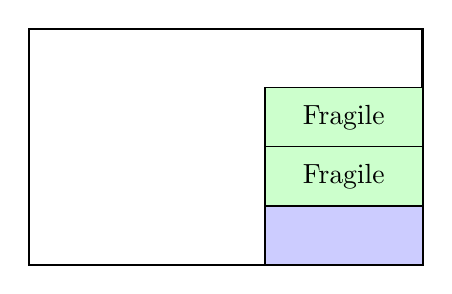
\begin{tikzpicture}
            % Draw the container
            \draw[thick] (0,0) rectangle (5,3);

            % Draw the three items inside
            \draw[fill=blue!20] (3,0) rectangle (5,0.75);
            \node at (4, 0.5) {};

            \draw[fill=green!20] (3,0.75) rectangle (5,1.5);
            \node at (4, 1.125) {Fragile};

            \draw[fill=green!20] (3,1.5) rectangle (5, 2.25);
            \node at (4, 1.875) {Fragile};

        \end{tikzpicture}
        \caption{Feasible stacking of items}
    \end{subfigure}
    \hfill
    % Second TikZ picture
    \begin{subfigure}[b]{0.45\textwidth}
        \centering
        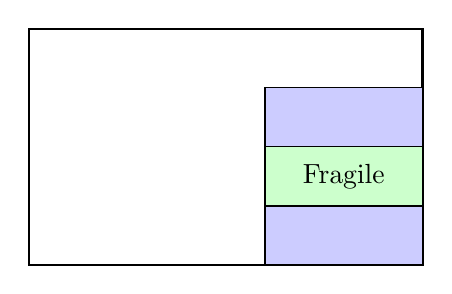
\begin{tikzpicture}
            \draw[thick] (0,0) rectangle (5,3);

            % Draw the three items inside
            \draw[fill=blue!20] (3,0) rectangle (5,0.75);
            \node at (4, 0.5) {};

            \draw[fill=green!20] (3,0.75) rectangle (5,1.5);
            \node at (4, 1.125) {Fragile};

            \draw[fill=blue!20] (3,1.5) rectangle (5, 2.25);
            \node at (4, 1.875) {};
        \end{tikzpicture}
        \caption{Infeasible stacking of items}
    \end{subfigure}
    \caption[Visualization fragile stacking]{Comparison fragile stacking \footnotemark}
    \footnotetext{Own figure}
    \label{fig:stacking_comparison}
\end{figure}


\subsubsection{Cargo-Related Constraints}
In contrast to item-related constraints, cargo-related constraints apply to
the entire cargo or to specific subsets of it. The \textbf{complete-shipment} constraint
requires that all items within a shipment must either be loaded into the same
container or be left behind entirely. This constraint is especially important
when container capacity is limited (\textit{output maximization}) and items
cannot be split. The \textbf{allocation constraint} serves a similar purpose.
It includes the \textbf{connectivity constraint}, which mandates that
certain items must be loaded into the same container, and the
\textbf{separation constraint}, which requires specific items to
be distributed across different containers. For example, kitchen
shipments, comprising multiple packages-should be delivered together
to enable efficient installation. Conversely, items such as perfume and fresh
vegetables should be shipped separately due to incompatibility.

\subsubsection{Positioning constraints}

Positioning constraints in container loading determine where items can be placed,
either absolute or relative to other items. The absolute positioning constraints specify
that certain items
must (or must not) be placed in specific areas of the container. These are
typically based on item characteristics such as size, weight, or
content (e.g., bulky or hazardous items placed near the container door for accessibility) or
exist in general for all item types, as the \textbf{geometry} and
\textbf{orthogonality} constraints. These constraints define that items are not allowed to overlap
and must be placed orhogonally to the container walls respectively.
Relative positioning constraints govern how items are arranged in
relation to each other. Either close to each other as \textit{group} or
\textit{separate} from each other. This differentiation is similar to the
\textit{allocation constraint} of the cargo-related constraints, but considers
only one container.
The \textbf{multi-drop constraints} combine
absolute and relative positioning requirements when items are destined for
different delivery locations. These constraints aim to minimize reloading
efforts by grouping items by delivery destination, by arranging item groups
in accordance with the delivery sequence and/or by applying a
\textbf{\gls{LIFO}} or \textbf{sequential loading policy}
to ensure efficient unloading without moving unrelated items. Adaptions of the \gls{LIFO} constraint,
consider either, that the items can be unpacked manually (\textbf{\gls{MLIFO}}) or can be unloaded generally
with a maximum distance to the unloading point (\textbf{reachability constraint}). These
types of positioning constraints are widely applied in the iterature due
to their practical relevance in real-world logistics operations.

\subsubsection{Load-related constraints}

The \textbf{stability constraint} is defined as one of the most critical constraints
in the \gls{CLP}, as it directly impacts
the safety of both the cargo and the personnel involved. First, a distinction
must be made between \textit{horizontal} and \textit{vertical} stability.
Horizontal stability is achieved when items are securely connected to the
container walls or to other items, preventing lateral movement. Vertical
stability, on the other hand, is defined in various ways throughout the
literature. One common approach evaluates the supporting area — the portion
of an item's base that rests on the surface below. Stability is often
considered sufficient if the support area covers between 70\% and 100\% of the base
of the item stacked on top. However, this can still cause unstable
configurations (see Figure~\ref{fig:vertical_stability_comparison}). To address this,
a more robust definition of vertical stability involves the consideration of a minimum support area
of all items below to avoid tilting of the cargo (\textbf{Robust Stability}). It is also essential to
ensure that the load remains stable even after parts of the cargo have been
unloaded. In addition, \textbf{complexity constraints} refer to specialized
requirements that are beyond standard packing rules. These include,
for example, compatibility with automated or robot-assisted packing systems.

\begin{figure}[htbp]
    \centering
    % First TikZ picture
    \begin{subfigure}[b]{0.45\textwidth}
        \centering
        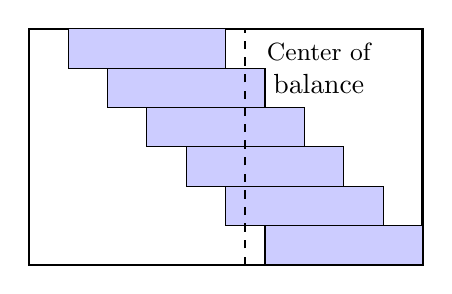
\begin{tikzpicture}
            % Draw the container
            \draw[thick] (0,0) rectangle (5,3);

            % Draw the three items inside
            \draw[fill=blue!20] (3,0) rectangle (5,0.5);
            \draw[fill=blue!20] (2.5,0.5) rectangle (4.5,1);
            \draw[fill=blue!20] (2,1) rectangle (4, 1.5);
            \draw[fill=blue!20] (1.5,1.5) rectangle (3.5, 2);
            \draw[fill=blue!20] (1,2) rectangle (3, 2.5);
            \draw[fill=blue!20] (0.5,2.5) rectangle (2.5, 3);
            %\node at (4, 1.875) {Fragile};
            \draw[thick,dashed] (2.75,0) -- (2.75,3);  % <---
            \node[anchor = west,align=center] at (2.9,2.5) {\small Center of \\  balance};

        \end{tikzpicture}
        \caption[align = center]{Feasible stacking with 75\% support area; infeasible due to unstable center}
    \end{subfigure}
    \hfill
    % Second TikZ picture
    \begin{subfigure}[b]{0.45\textwidth}
        \centering
        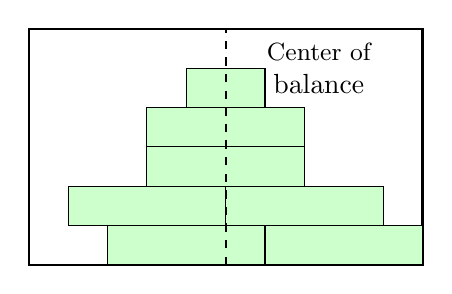
\begin{tikzpicture}
            % Draw the container
            \draw[thick] (0,0) rectangle (5,3);

            % Draw the three items inside
            \draw[fill=green!20] (3,0) rectangle (5,0.5);
            \draw[fill=green!20] (1,0) rectangle (3,0.5);

            \draw[fill=green!20] (2.5,0.5) rectangle (4.5,1);
            \draw[fill=green!20] (0.5,0.5) rectangle (2.5,1);

            \draw[fill=green!20] (1.5,1) rectangle (3.5, 1.5);
            \draw[fill=green!20] (1.5,1.5) rectangle (3.5, 2);
            \draw[fill=green!20] (2,2) rectangle (3, 2.5);

            \draw[thick,dashed] (2.5,0) -- (2.5,3);  % <---
            \node[anchor = west,align=center] at (2.9,2.5) {\small Center of \\  balance};
        \end{tikzpicture}
        \caption[align = center]{Feasible stacking regarding 75\% support area and stable center}
    \end{subfigure}
    \caption[Visualization vertical stability]{Comparison vertical stability (side view) \footnotemark}
    \footnotetext{Own figures based on \cite[p.845]{krebs_advanced_2021}}
    \label{fig:vertical_stability_comparison}
\end{figure}
